\section{Results - Research Question 2}

\subsection{Comparing Existing Work}

\begin{figure}[h]
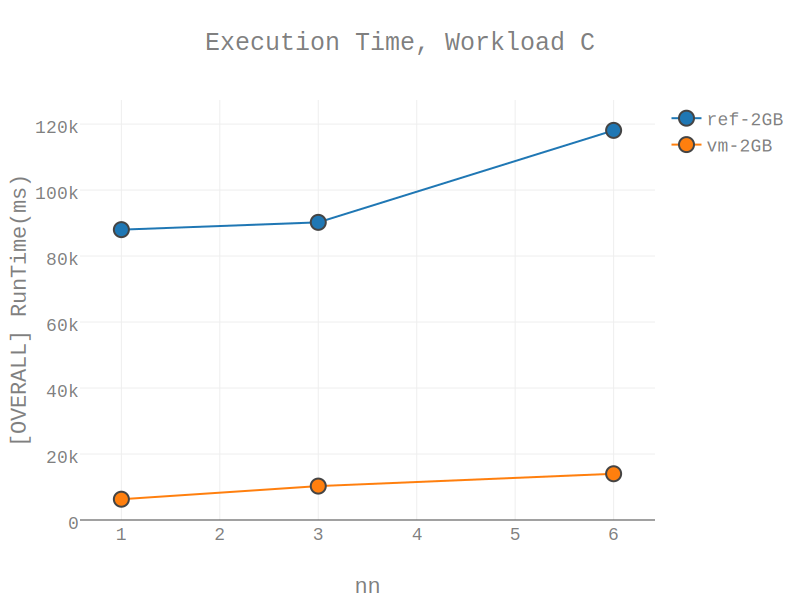
\includegraphics[width=3.5in]{Figures/figures-wlc_fig5.pdf}

\caption{Comparing the results in \cite{Abramova2014} with the median value of the virtual machine assigned 2GB of \gls{ram}.  Note that the virtual machines were on a nodal network (minimal propagation delay) while the the links in \cite{Abramova2014} were unspecified.}

\label{fig:figures-wlc_fig5}
\end{figure}

Here, as depicted in \ref{fig:figures-wlc_fig5}, one can see that the virtual machine configured to represent the network in \cite{Abramova2014} appears to perform at a significantly shorter execution time compared to the work done in \cite{Abramova2014}, probably largely due to the fact that the networks are nodal and do not experience any significant propagation delay compared, what could be inferred to be, a physical Ethernet cable.

The summary for the 2GB virtual node are in Tables \ref{table:summary_statistics_for_1_config}, \ref{table:summary_statistics_for_3_config}, and \ref{table:summary_statistics_for_6_config} under 'ram2GB'.  

One would expect, given that once this is extended to the Raspberry Pi modules require some kind of physical network connection (Ethernet) and a 900 MHz processor compared to the 2.90 GHz processor used by the virtual machines, the performance would be represented by significantly longer execution time.  

Facing minimal propagation delay due to being connected on a nodal network, experiments with the virtual machines seek to place an upper limit on potential \gls{iot} performance expectations, which for this analysis translates to a floor on timing.  Additional conventions would be necessary to find any sort of universal floor on Cassandra, but for the experiments, the results from running experiments on the virtual machines.

\subsection{Testing various memory sizes}

We now discuss testing and performance for memory sizes ranging from 1GB to 4GB.  The experience with 512MB was documented with Workload A.

\subsubsection{Experimental Testing for Memory in the 1GB – 4GB Range}

This section describes the results of running the \gls{ycsb} on virtual node networks as described in the methodology.  The summary of execution times are reported in Tables \ref{table:summary_statistics_for_1_config}, \ref{table:summary_statistics_for_3_config}, and \ref{table:summary_statistics_for_6_config}.  For each table, the summary statistics are listed for each amount of memory.

\paragraph{Visual Inspection of Results}

It is best to start with a visual inspection of the data represented in Figure \ref{fig:figures-wlc_fig4}.  Generally the greater amount of \gls{ram}, the fewer problems one would have with memory overloads, or needing to compact. However, for each sample, it seems that different amount of memory yields the best performance.

If there was a hint that 4GB performs better than 2GB, or 2GB performs better than 1GB, or both, this might be cause to attempt a regression to form a preliminary predictive model.  However, from first glance, it appears that an further examination of the data will indicate that the amount of memory does not independently predict performance, forming the null hypothesis of the \gls{anova} test to come.

\begin{figure}[h]
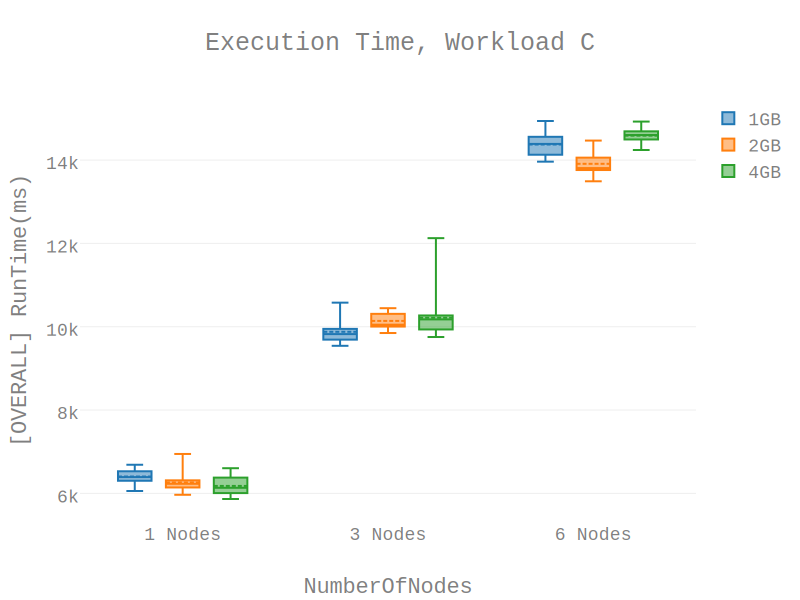
\includegraphics[width=3.5in]{Figures/figures-wlc_fig4.pdf}

\caption{Execution time for virtual machines with 1GB, 2GB, and 4GB of \gls{ram}.  The first 9 trials have been removed in order to filter out the trials representing the cache effect and thus represent the steady state.}

\label{fig:figures-wlc_fig4}
\end{figure}
\begin{table}
\begin{tabular}{lrrr}
\toprule
 index &  ram1GB &  ram2GB &  ram4GB \\
\midrule
 count &      21 &      21 &      21 \\
  mean & 6404.62 & 6263.71 &    6179 \\
   std & 165.241 & 221.031 & 231.934 \\
   min &    6057 &    5966 &    5865 \\
   25\% &    6304 &    6152 &    6017 \\
   50\% &    6391 &    6230 &    6134 \\
   75\% &    6526 &    6306 &    6377 \\
   max &    6687 &    6946 &    6604 \\
 range &     630 &     980 &     739 \\
\bottomrule
\end{tabular}
\caption{Summary Statistics for 1-Node Configuration. All values represented fall between 5865.0 ms and 6946.0 ms, or rather within a span of 1081.0 ms.}
\label{table:summary_statistics_for_1_config}
\end{table}
\begin{table}
\begin{tabular}{lrrr}
\toprule
 index &  ram1GB &  ram2GB &  ram4GB \\
\midrule
 count &      21 &      21 &      21 \\
  mean & 9878.24 & 10139.6 & 10215.5 \\
   std & 255.122 & 180.863 & 495.567 \\
   min &    9542 &    9849 &    9753 \\
   25\% &    9695 &   10009 &    9935 \\
   50\% &    9823 &   10049 &   10176 \\
   75\% &    9929 &   10307 &   10263 \\
   max &   10578 &   10445 &   12126 \\
 range &    1036 &     596 &    2373 \\
\bottomrule
\end{tabular}
\caption{Summary Statistics for 3-Node Configuration. All values represented fall between 9542.0 ms and 12126.0 ms, or rather within a span of 2584.0 ms.}
\label{table:summary_statistics_for_3_config}
\end{table}
\begin{table}
\begin{tabular}{lrrr}
\toprule
 index &  ram1GB &  ram2GB &  ram4GB \\
\midrule
 count &      21 &      21 &      21 \\
  mean & 14373.4 & 13910.4 & 14586.3 \\
   std & 302.838 & 263.331 & 180.081 \\
   min &   13962 &   13491 &   14242 \\
   25\% &   14137 &   13763 &   14496 \\
   50\% &   14388 &   13808 &   14601 \\
   75\% &   14551 &   14020 &   14690 \\
   max &   14938 &   14468 &   14924 \\
 range &     976 &     977 &     682 \\
\bottomrule
\end{tabular}
\caption{Summary Statistics for 6-Node Configuration. All values represented fall between 13491.0 ms and 14938.0 ms, or rather within a span of 1447.0 ms.}
\label{table:summary_statistics_for_6_config}
\end{table}

\paragraph{Absolute Ranges}

While Figure \ref{fig:figures-wlc_fig4} gives a general sense of what the results look like, the actual summary statistics can be examined in Tables \ref{table:summary_statistics_for_1_config}, \ref{table:summary_statistics_for_3_config}, and \ref{table:summary_statistics_for_6_config}. After filtering out the first nine trials, the results for running 10,000 operations is displayed in Tables \ref{table:summary_statistics_for_1_config}, \ref{table:summary_statistics_for_3_config}, and \ref{table:summary_statistics_for_6_config}.  For each configuration, varying the \gls{ram} of the virtual machine resulted in execution times that fell within 2 seconds of each other.

\paragraph{\gls{anova}}

A one-way \gls{anova} was performed with the filtered data, and the \gls{anova} summary tables can be seen in Tables \ref{ram_variance_analysis_workload_a_1_node}, \ref{ram_variance_analysis_workload_a_3_node}, and \ref{ram_variance_analysis_workload_a_6_node} for the 1, 3, and 6 node cases respectively.  For each case, the  p-value is much, much less than 0.05, and thus it can be said that one can be 95\% confident in the decision to fail to reject the null hypothesis, the hypothesis that the means are equal.

\begin{table}
\begin{tabular}{lrrrrr}
\toprule
         Source &            SS &  df &             MS &         F &         p \\
\midrule
 between groups &  5.455423e+05 &   2 &  272771.158730 &  6.297012 &  0.003292 \\
  within groups &  2.599053e+06 &  60 &   43317.553968 &       NaN &       NaN \\
          total &  3.144596e+06 &  62 &            NaN &       NaN &       NaN \\
\bottomrule
\end{tabular}
\caption{ANOVA Summary Table for Workload C, 1 Node}
\label{table:ram_variance_analysis_workload_c_1_node}
\end{table}

\begin{table}
\begin{tabular}{lrrrrr}
\toprule
         Source &            SS &  df &             MS &         F &         p \\
\midrule
 between groups &  1.314779e+06 &   2 &  657389.349207 &  5.743313 &  0.005221 \\
  within groups &  6.867702e+06 &  60 &  114461.703175 &       NaN &       NaN \\
          total &  8.182481e+06 &  62 &            NaN &       NaN &       NaN \\
\bottomrule
\end{tabular}
\caption{ANOVA Summary Table for Workload C, 3 Node}
\label{table:ram_variance_analysis_workload_c_3_node}
\end{table}

\begin{table}
\begin{tabular}{lrrrrr}
\toprule
         Source &            SS &  df &            MS &          F &             p \\
\midrule
 between groups &  5.015054e+06 &   2 &  2.507527e+06 &  38.879796 &  1.482116e-11 \\
  within groups &  3.869660e+06 &  60 &  6.449434e+04 &        NaN &           NaN \\
          total &  8.884714e+06 &  62 &           NaN &        NaN &           NaN \\
\bottomrule
\end{tabular}
\caption{ANOVA Summary Table for Workload C, 6 Node}
\label{table:ram_variance_analysis_workload_c_6_node}
\end{table}

Examining the effects of variance in the amount of \gls{ram} allocated the virtual machines does not seem to have a notable impact on performance.  This indicates that, any observed limitation on the Raspberry Pis’ performance is not limited by \gls{ram}, but something else, and that varying \gls{ram} in future tests will not yield significant results.

% Insert something about statistical significance

\subsection{Implementation on Raspberry Pi}

In a similar fashion, the tests were run on the Raspberry Pi to observe performance.  The spread of each of the tests can be seen in Figure \ref{fig:wlc_fig10} and Table \ref{table:wired-results}.  The results, next to one trend for the virtual machines, can be seen in Figure \ref{fig:fig06}. 

\begin{figure}[h]
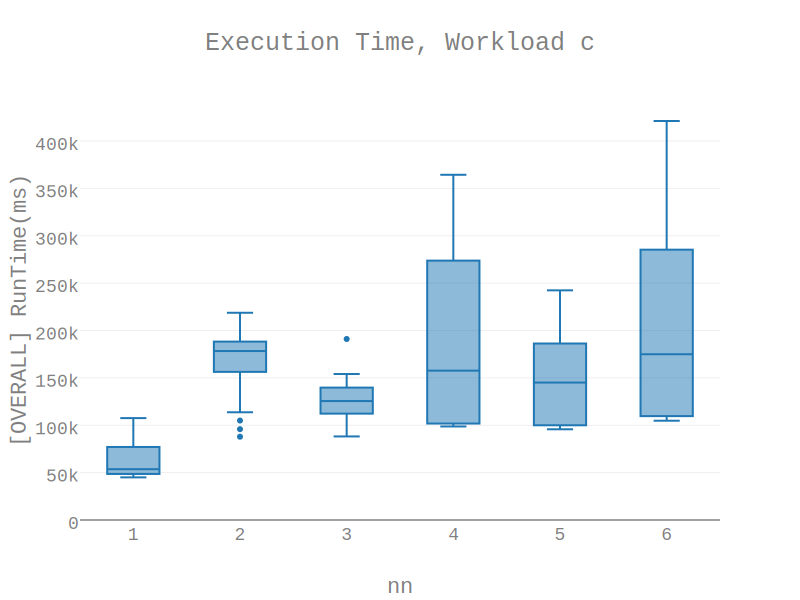
\includegraphics[width=3.5in]{Figures/figures-wlc_fig10.pdf}

\caption{Box plot representing the results of the workload applied to wired local area network on the Raspberry Pi platform.}

\label{fig:wlc_fig10}
\end{figure}

\begin{figure}[h]
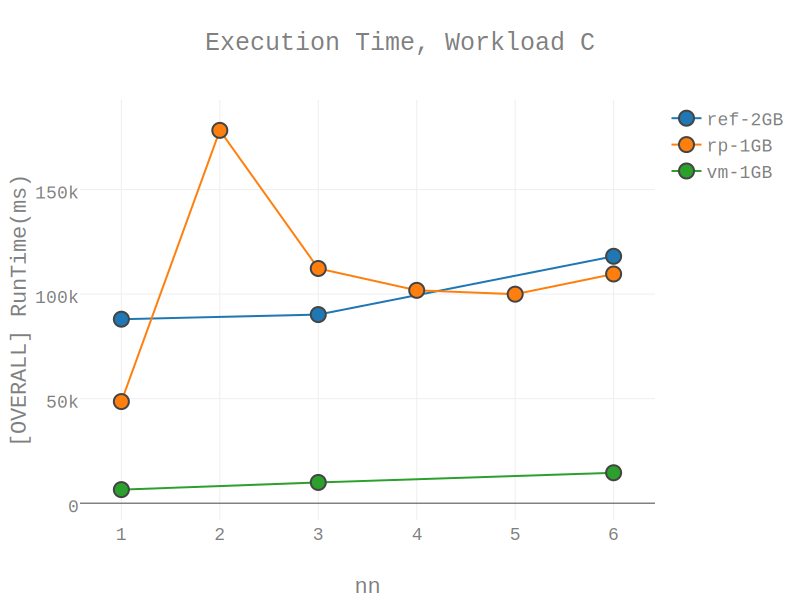
\includegraphics[width=3.5in]{Figures/figures-wlc_fig6.pdf}

\caption{Comparison between the Raspberry Pi nodes (rp-1GB), the results reported in \cite{Abramova2014} (ref-2GB), and the virtual nodes with 4GB available \gls{ram} (vm-4GB).}

\label{fig:fig06}
\end{figure}

\begin{table}
\begin{tabular}{lrrr}
\toprule
 index &       1 &       3 &       6 \\
\midrule
 count &      21 &      21 &      21 \\
  mean & 4.8e+04 & 1.1e+05 & 1.1e+05 \\
   std & 1.8e+03 & 3.2e+03 & 2.1e+03 \\
   min & 4.5e+04 & 1.1e+05 &   1e+05 \\
   25\% & 4.7e+04 & 1.1e+05 & 1.1e+05 \\
   50\% & 4.9e+04 & 1.1e+05 & 1.1e+05 \\
   75\% &   5e+04 & 1.1e+05 & 1.1e+05 \\
   max &   5e+04 & 1.3e+05 & 1.1e+05 \\
 range & 5.4e+03 & 1.7e+04 & 8.1e+03 \\
\bottomrule
\end{tabular}
\caption{Summary for Raspberry Pi wired local area network}
\label{table:rp_wired_summary_statistics}
\end{table}

As can be seen from Figure \ref{fig:fig06}, the Raspberry Pi configuration takes considerably more execution time than the virtual machine analogy, which is probably due to the physical nature of the Ethernet connections (propagation delay) and the I/O limitations of the Raspberry Pi hardware.  However, its seemingly similar performance to the reference in \cite{Abramova2014} suggests the \gls{io} for the \gls{sd} Card follows a predictable pattern, and actually seems to outperform the node in \cite{Abramova2014} in the degenerate 1-node case.

For this paragraph, consider the results from \cite{Abramova2014} as the reference.  For a node network of 1, the experimental values fell between 43260.0 ms and 48123.0 ms, inclusive, and all values fell within 15170.0 ms of the reference value of 58430 ms.  For a node network of 3, the experimental values fell between 93702.0 ms and 100501.0 ms, inclusive, and all values fell within 34851.0 ms of the reference value of 65650 ms.  For a node network of 6, the experimental values fell between 103728.0 ms and 111002.0 ms, inclusive, and all values fell within 23692.0 ms of the reference value of 87310 ms.  

\subsection{Wireless Links}

The median value of the corresponding wired experiment will serve as the reference in this paragraph. For a node network of 1, the experimental values fell between 74072.0 ms and 119580.0 ms, inclusive, and all values fell within 73961.0 ms of the reference value of 45619.0 ms.  For a node network of 3, the experimental values fell between 123064.0 ms and 149252.0 ms, inclusive, and all values fell within 52156.0 ms of the reference value of 97096.0 ms.  For a node network of 6, the experimental values fell between 246945.0 ms and 355538.0 ms, inclusive, and all values fell within 248820.0 ms of the reference value of 106718.0 ms.

\begin{figure}[h]
\includegraphics[width=3.5in]{Figures/figures-wlc_fig7.pdf}

\caption{Comparison between the Ethernet links (eth) and wireless links (wlan) using the Raspberry Pi nodes.}

\label{fig:fig07}
\end{figure}

Figure \ref{fig:fig07} depicts the two experiments using Raspberry Pis: a wireless LAN (wlan) and an Ethernet LAN (eth).  In Figure \ref{fig:fig07}, as well as previous graphs, one can observe that the the Ethernet LAN effects about 50 seconds of execution time for 10,000 operations.  The initial median execution time for a node on a wireless LAN was found to be double the execution time.

For both configurations, performance takes a hit when transitioning from 1 to 2 nodes, but then increases from 2 nodes to 3 nodes.  From 3 nodes to 4 nodes, the wireless LAN configuration’s performance decreases dramatically, compared to slight increase in the wired Ethernet case.  

\begin{figure}[h]
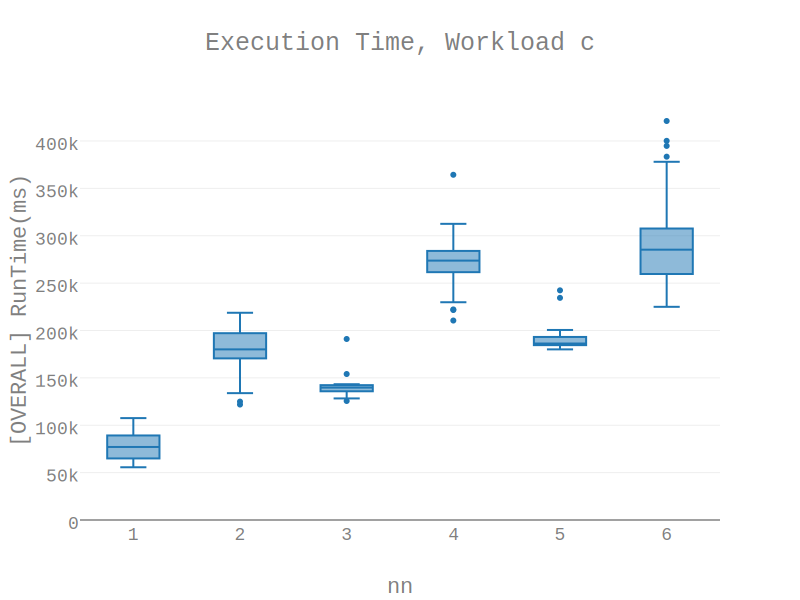
\includegraphics[width=3.5in]{Figures/figures-wlc_fig8.pdf}

\caption{Distribution for all 30 trials of execution times where the Raspberry Pi nodes were connected via a wireless \gls{lan}.  Suspected outliers, values more than 3 times the interquartile range, are included as individual points above and below the 'maximum' and 'minimum' bars.}

\label{fig:fig08}
\end{figure}

A summary representation box plot of the results of wireless experimentation is above.  Here, the laptop was connected to the router via an Ethernet cable, and each node was connected to the router on a wireless local area network (LAN).  Suspected outliers, values more than 3 times the interquartile range (IQR) are included as points above and below.
There seems to be an overall increasing trend, while the data seems to oscillate, performing better for odd (1,3,5 node) configurations than for even (2,4,6 node) configurations.  However, there is no current theory behind this anomaly. 

\begin{figure}[h]
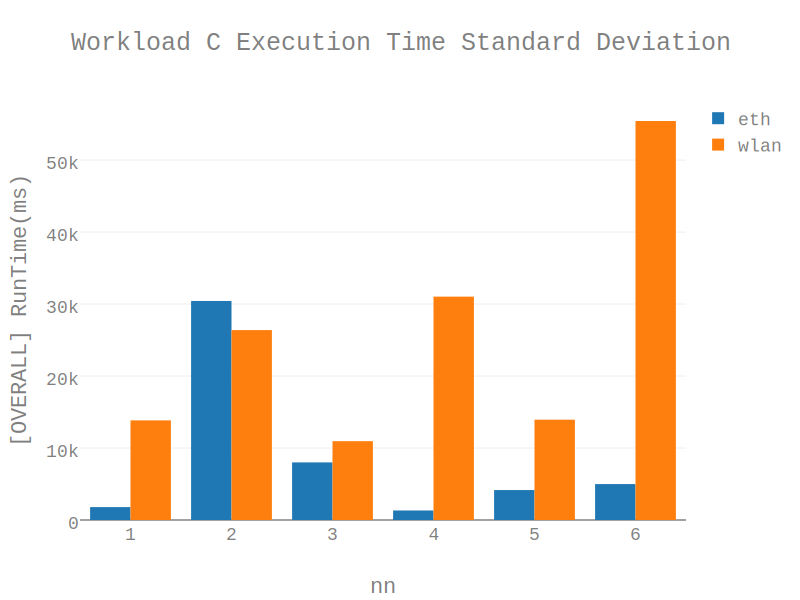
\includegraphics[width=3.5in]{Figures/figures-wlc_fig9.pdf}

\caption{This compares the standard deviation in execution times for 10,000 operations of Workload C on the wired (eth) versus the wireless (wlan) configurations for 1 node, 2 nodes, 3 nodes, up through 6 nodes in milliseconds.}

\label{fig:fig09}
\end{figure}

To supplement the box plot, the standard deviation execution times for each set of trials, separated by number of nodes, is depicted in Figure \ref{fig:fig09}.  The difference seen here appears stark, and is overwhelming compared to the variance between 1, 2, 3, 4, 5 and 6 node networks given the same communication method. 

%1)      Reduced performance of Workload A is not statistically significant for the reduced memory sizes of IoT like devices
%2)      When varying platforms, performance for Workload A tracks the performance of the reference paper. For trials performe, reduced performance of Workload A is within 100ms of the reference paper (abramova) for wired implementations.
%3)      When varying communication method, reduced performance of Workload A is within 100ms of the wired platform test (order of magnitude, no greater than 100% increase in delay)
%4)      Reduced performance of Workload C is not statistically significant for the reduced memory sizes of IoT like devices
%5)      When varying platforms, reduced performance of Workload C is within 100ms of the reference paper (abramova) for wired implementations
%6)      When varying communication method, reduced performance of Workload C is within 100ms of the wired platform test
%7)      Reduced performance of Workload E is not statistically significant for the reduced memory sizes of IoT like devices
%8)      When varying platforms, reduced performance of Workload E is within 100ms of the reference paper (abramova) for wired implementations
%9)      When varying communication method, reduced performance of Workload E is within 100ms of the wired platform test
